%%%%%%%%%%%%%%%%%%%%%%%%%%%%%%%%%%%%%
%% Supporting Information
%% (Optional)
%%%%%%%%%%%%%%%%%%%%%%%%%%%%%%%%%%%%%
% OVERVIEW
%
% Please note that all supporting information will be peer reviewed with your manuscript.
% In general, the purpose of the supporting information is to enable
% authors to provide and archive auxiliary information such as data
% tables, method information, figures, video, or computer software,
% in digital formats so that other scientists can use it.

% The key criteria are that the data:
% 1. supplement the main scientific conclusions of the paper but are not essential to the conclusions (with the exception of
%    including data so the experiment can be reproducible);
% 2. are likely to be usable or used by other scientists working in the field;
% 3. are described with sufficient precision that other scientists can understand them, and
% 4. are not exe files.
%

% All Supporting text and figures should be included in this document.

% Data sets, large tables, movie files,
% and audio files should be uploaded separately, following AGU naming
% conventions. Include their captions in this document and list the
% file name with the caption. You will be prompted to upload these
% files on the Upload Files tab during the submission process, using
% file type “Supporting Information (SI)”

\documentclass[draft]{agujournal}

% Please type in the journal name: \journalname{<Journal Name>}
% ie,
\journalname{Journal of Advances in Modeling Earth Systems (JAMES)}

%% Choose from this list of Journals:
%
% Journal of Geophysical Research
% JGR-Biogeosciences
% JGR-Earth Surface
% JGR-Planets
% JGR-Solid Earth
% JGR-Space Physics
% Global Biochemical Cycles
% Geophysical Research Letters
% Paleoceanography
% Radio Science
% Reviews of Geophysics
% Tectonics
% Space Weather
% Water Resource Research
% Geochemistry, Geophysics, Geosystems
% Journal of Advances in Modeling Earth Systems (JAMES)
% Earth's Future
% Earth and Space Science

\begin{document}

%% This command needs article title as argument to \supportinginfo{}:
\supportinginfo{Implementing plant hydraulics in the Community Land Model, version 5}

 \authors{Daniel Kennedy\affil{1},
Sean Swenson\affil{2},
Keith W. Oleson\affil{2},
David M. Lawrence\affil{2},
Rosie Fisher\affil{2},
Antonio Carlos Lola da Costa\affil{3},
Pierre Gentine\affil{1}}

\affiliation{1}{Columbia University, New York, NY 10027 USA}
\affiliation{2}{National Center for Atmospheric Research, Table Mesa Drive, Boulder, Colorado, USA}
\affiliation{3}{Centro de Geoci\^encias, Universidade Federal do Par\'a, Bel\'em, Par\'a, Brazil}
\correspondingauthor{Daniel Kennedy}{djk2120@columbia.edu}

%% ------------------------------------------------------------------------ %%
%
%  TEXT
%
%% ------------------------------------------------------------------------ %%

\section*{Contents}
%%%Remove or add items as needed%%%
\begin{enumerate}
\item Figures S1 to \ref{supp:cool}
\end{enumerate}


\section*{Figures}
\renewcommand{\thefigure}{S\arabic{figure}}

  \begin{figure}[h]
     \centering
     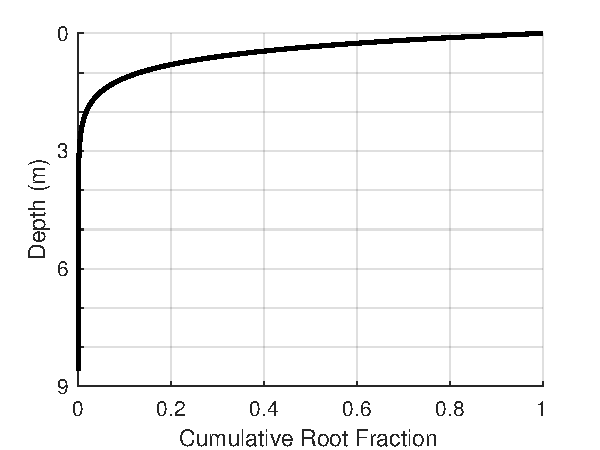
\includegraphics[width=20pc]{roots.pdf}
     \caption{Cumulative rooting distribution.}
     \label{roots}
  \end{figure}
         \clearpage
         
         
      \begin{figure}[h]
     \centering
     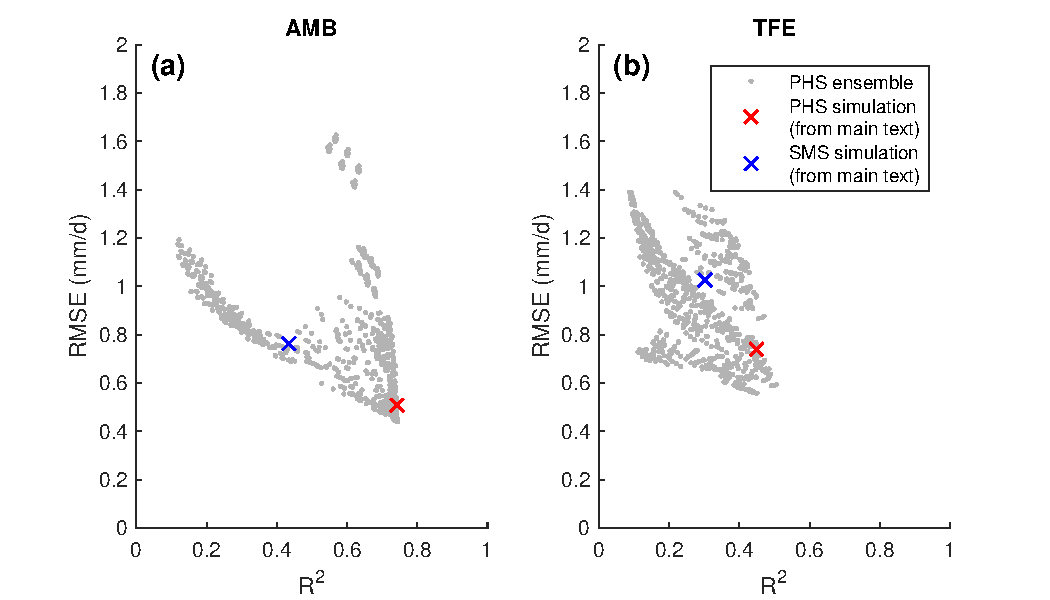
\includegraphics[width=30pc]{ens.pdf}
     \caption{Results of the PHS parameter tuning exercise. The main text PHS simulation was chosen to maximize R$^2$ - RMSE.
     }
     \label{supp:ens}
       \end{figure}


        \clearpage

    \clearpage   
      \begin{figure}[h]
     \centering
     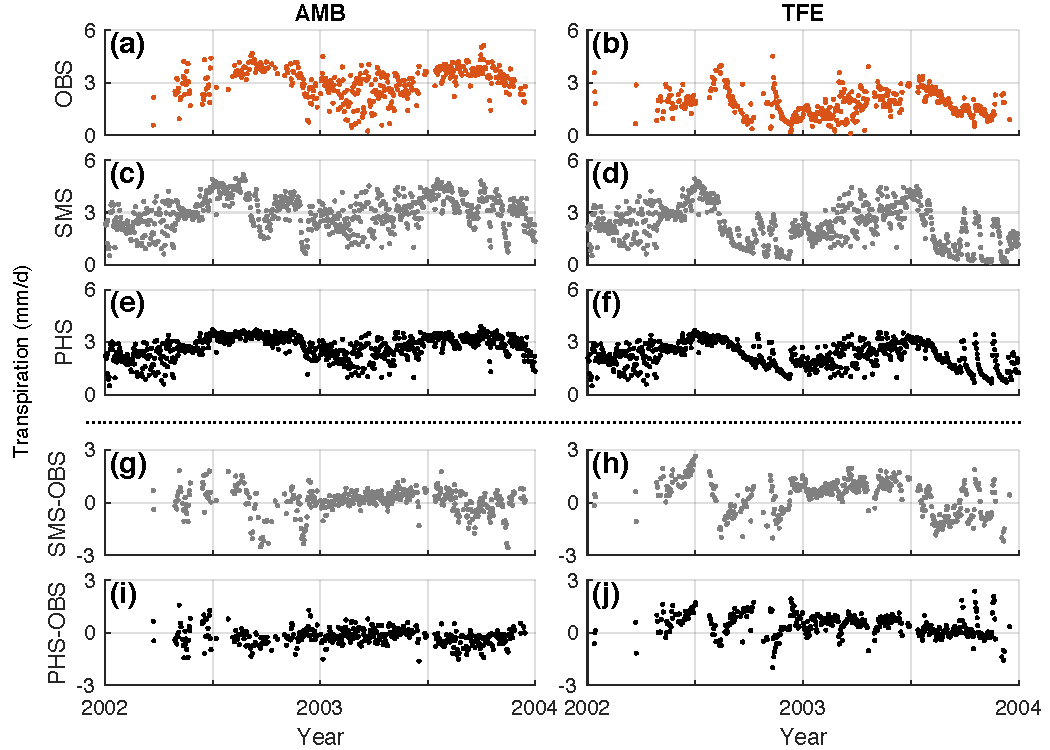
\includegraphics[width=30pc]{fctr_ts.pdf}
     \caption{(a-f) Time-series of daily total transpiration (mm/d), from (a,b) observations, (c,d) SMS model configuration, and (e,f) PHS model configuration under ambient and TFE conditions.
     
     (g-j) Difference between modeled and observed transpiration (mm/d), for (g,h) SMS and (i,j) PHS under ambient and TFE conditions.
     }
     \label{fig:t2}
  \end{figure}
    


    \begin{figure}[h]
     \centering
     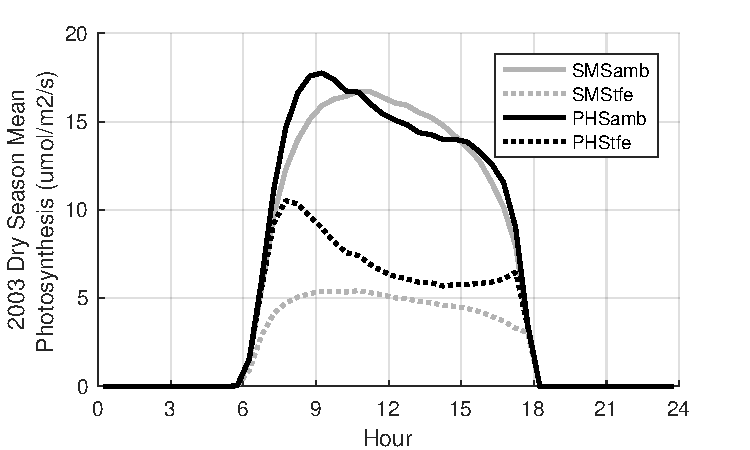
\includegraphics[width=20pc]{suppfpsn.pdf}
     \caption{2003 dry season diurnal mean photosynthesis under ambient and TFE conditions for the two model configurations.
     }
     \label{supp:fpsn}
  \end{figure}

\clearpage
    \begin{figure}[h]
     \centering
     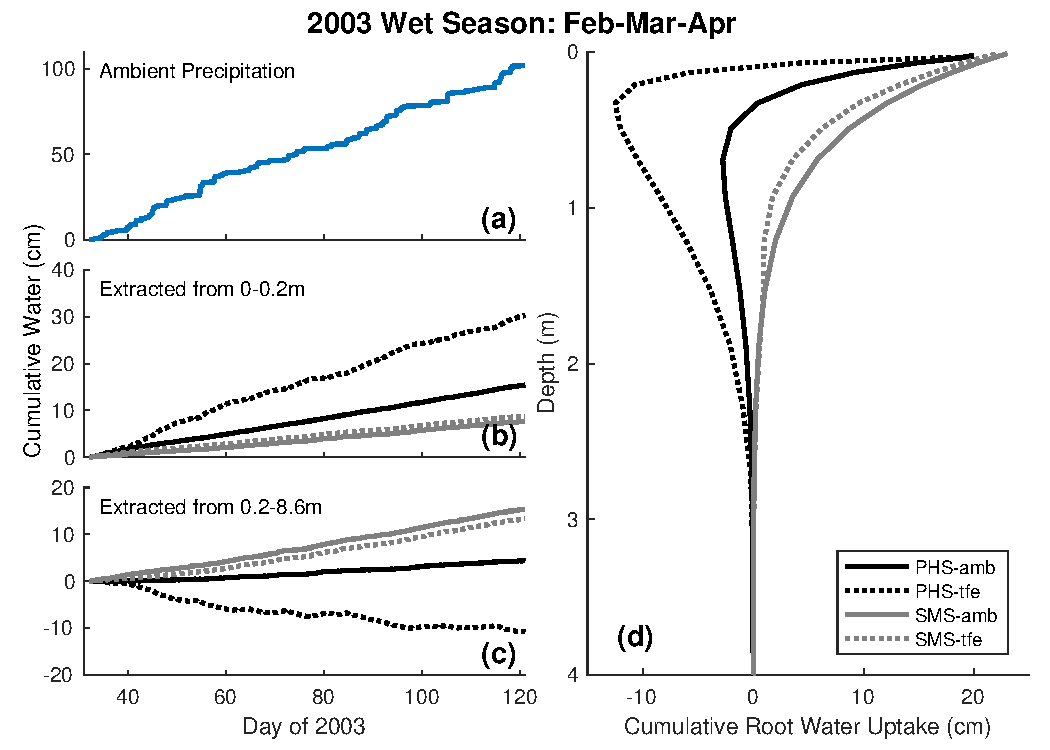
\includegraphics[width=30pc]{qwet.pdf}
     \caption{2003 wet season (FMA) cumulative root water uptake and precipitation. 
     (a) Cumulative precipitation over time under ambient conditions
     (b,c) Cumulative water uptake over time from above and below 0.2m, respectively.
     (d) Cumulative root water uptake with depth.
     }
     \label{fig:qwet}
  \end{figure}


      \begin{figure}[h]
     \centering
     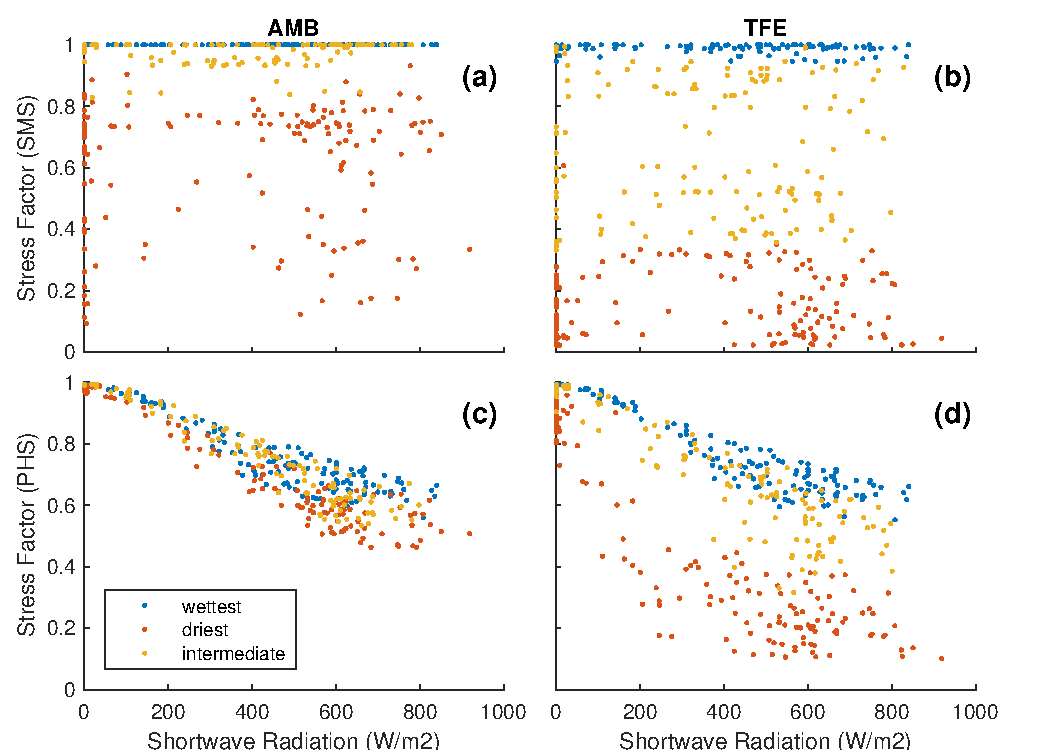
\includegraphics[width=30pc]{suppstress.pdf}
     \caption{Water stress factor versus downwelling shortwave radiation (2002-2003), for timesteps with VPD between 1 and 1.0559 kPa (n=470).
     VPD is controlled to highlight the relationship with downwelling radiation, the reverse (controlling for radiation) is shown in Figure 7.
     For SMS (a,b), data are subdivided based on average soil matric potential, weighted by root fraction.
     For PHS (c,d), data are subdivided based on predawn (5h) root water potential.
     Blue dots represent the wettest tercile, yellow dots represent the intermediate tercile, and red dots represent the driest tercile.
     }
     \label{supp:fsds}
       \end{figure}
         \clearpage

  
  \begin{figure}[h]
     \centering
     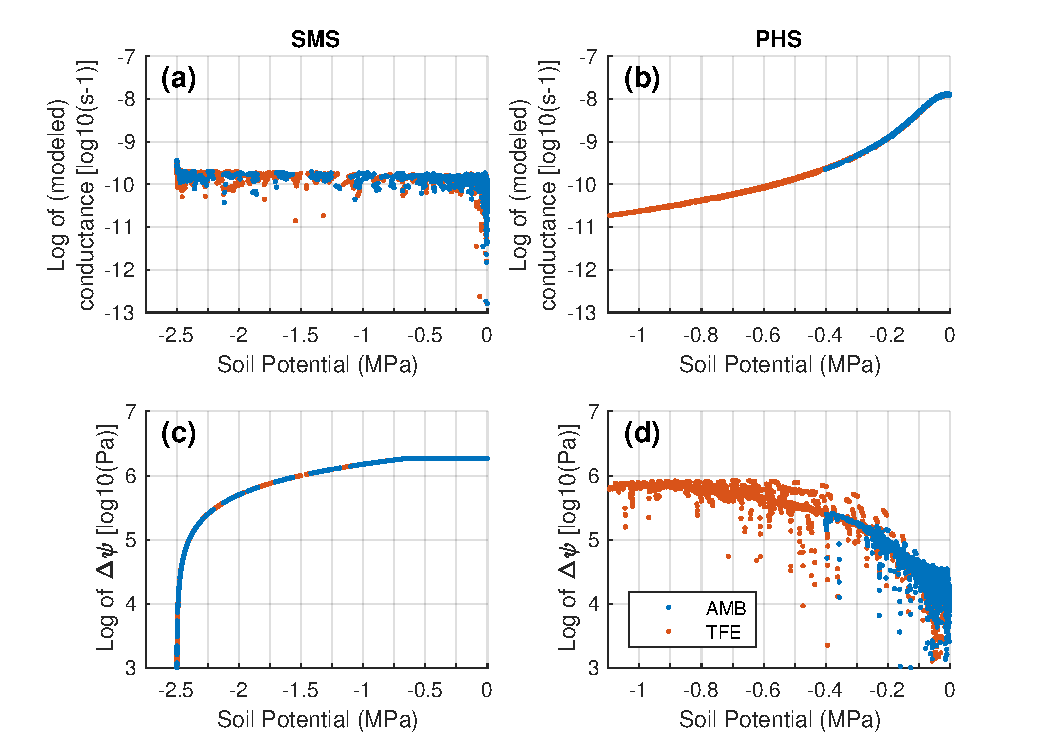
\includegraphics[width=30pc]{suppcond.pdf}
     \caption{(a,b) Log of conductance ($k_{s,r}$) versus soil potential for Soil Layer 5.
     (c,d) Log of hydraulic gradient ($\Delta\psi$) versus soil potential for Soil Layer 5.
     Note that the soil potential axes vary for PHS vs. SMS. 
     
     Multiplied together $k_{s,r}$ and $\Delta\psi$ yield the Layer-5 root water uptake.
     PHS conductance decreases by almost 3 orders of magnitude between 0 and -1MPa, which leads to reduced RWU, though this is offset (by about half) due to increases in $\Delta\psi$.
     
     
     while SMS $\Delta\psi$ decreases by less than 1 order of magnitude between 0 and -2MPa, 
     leading to higher sensitivity to soil potential with PHS, see Figure 10.
     
     Only midday (12h-14h, 2002-2003) timesteps are shown to emphasize the relationship with soil potential.
     With SMS, conductance is not modeled explicitly, but rather calculated as $k$=$q/\Delta\psi$ (see Section 2.4.2). 
     For soil potentials greater than or equal to 2.5MPa, $\Delta\psi$=0, and SMS implied conductance is undefined, but could probably be considered to equal 0.
     PHS conductance captures both root tissue and soil matrix resistances (operating in series).}
     \label{supp:cond}
  \end{figure}
  \clearpage
  
      \begin{figure}[h]
     \centering
     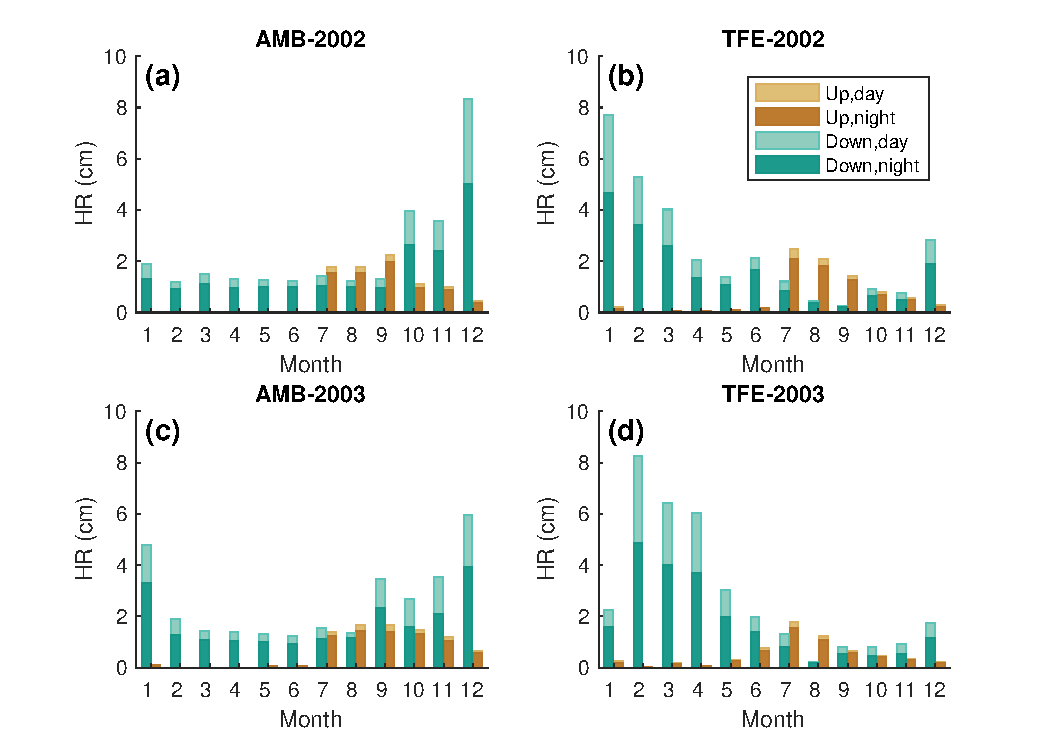
\includegraphics[width=30pc]{hr2.pdf}
     \caption{PHS hydraulic distribution during 2002 and 2003, partitioning by direction and time of day.}
     \label{supp:hr}
  \end{figure}
  \clearpage

  
        \clearpage
    \begin{figure}[h]
     \centering
     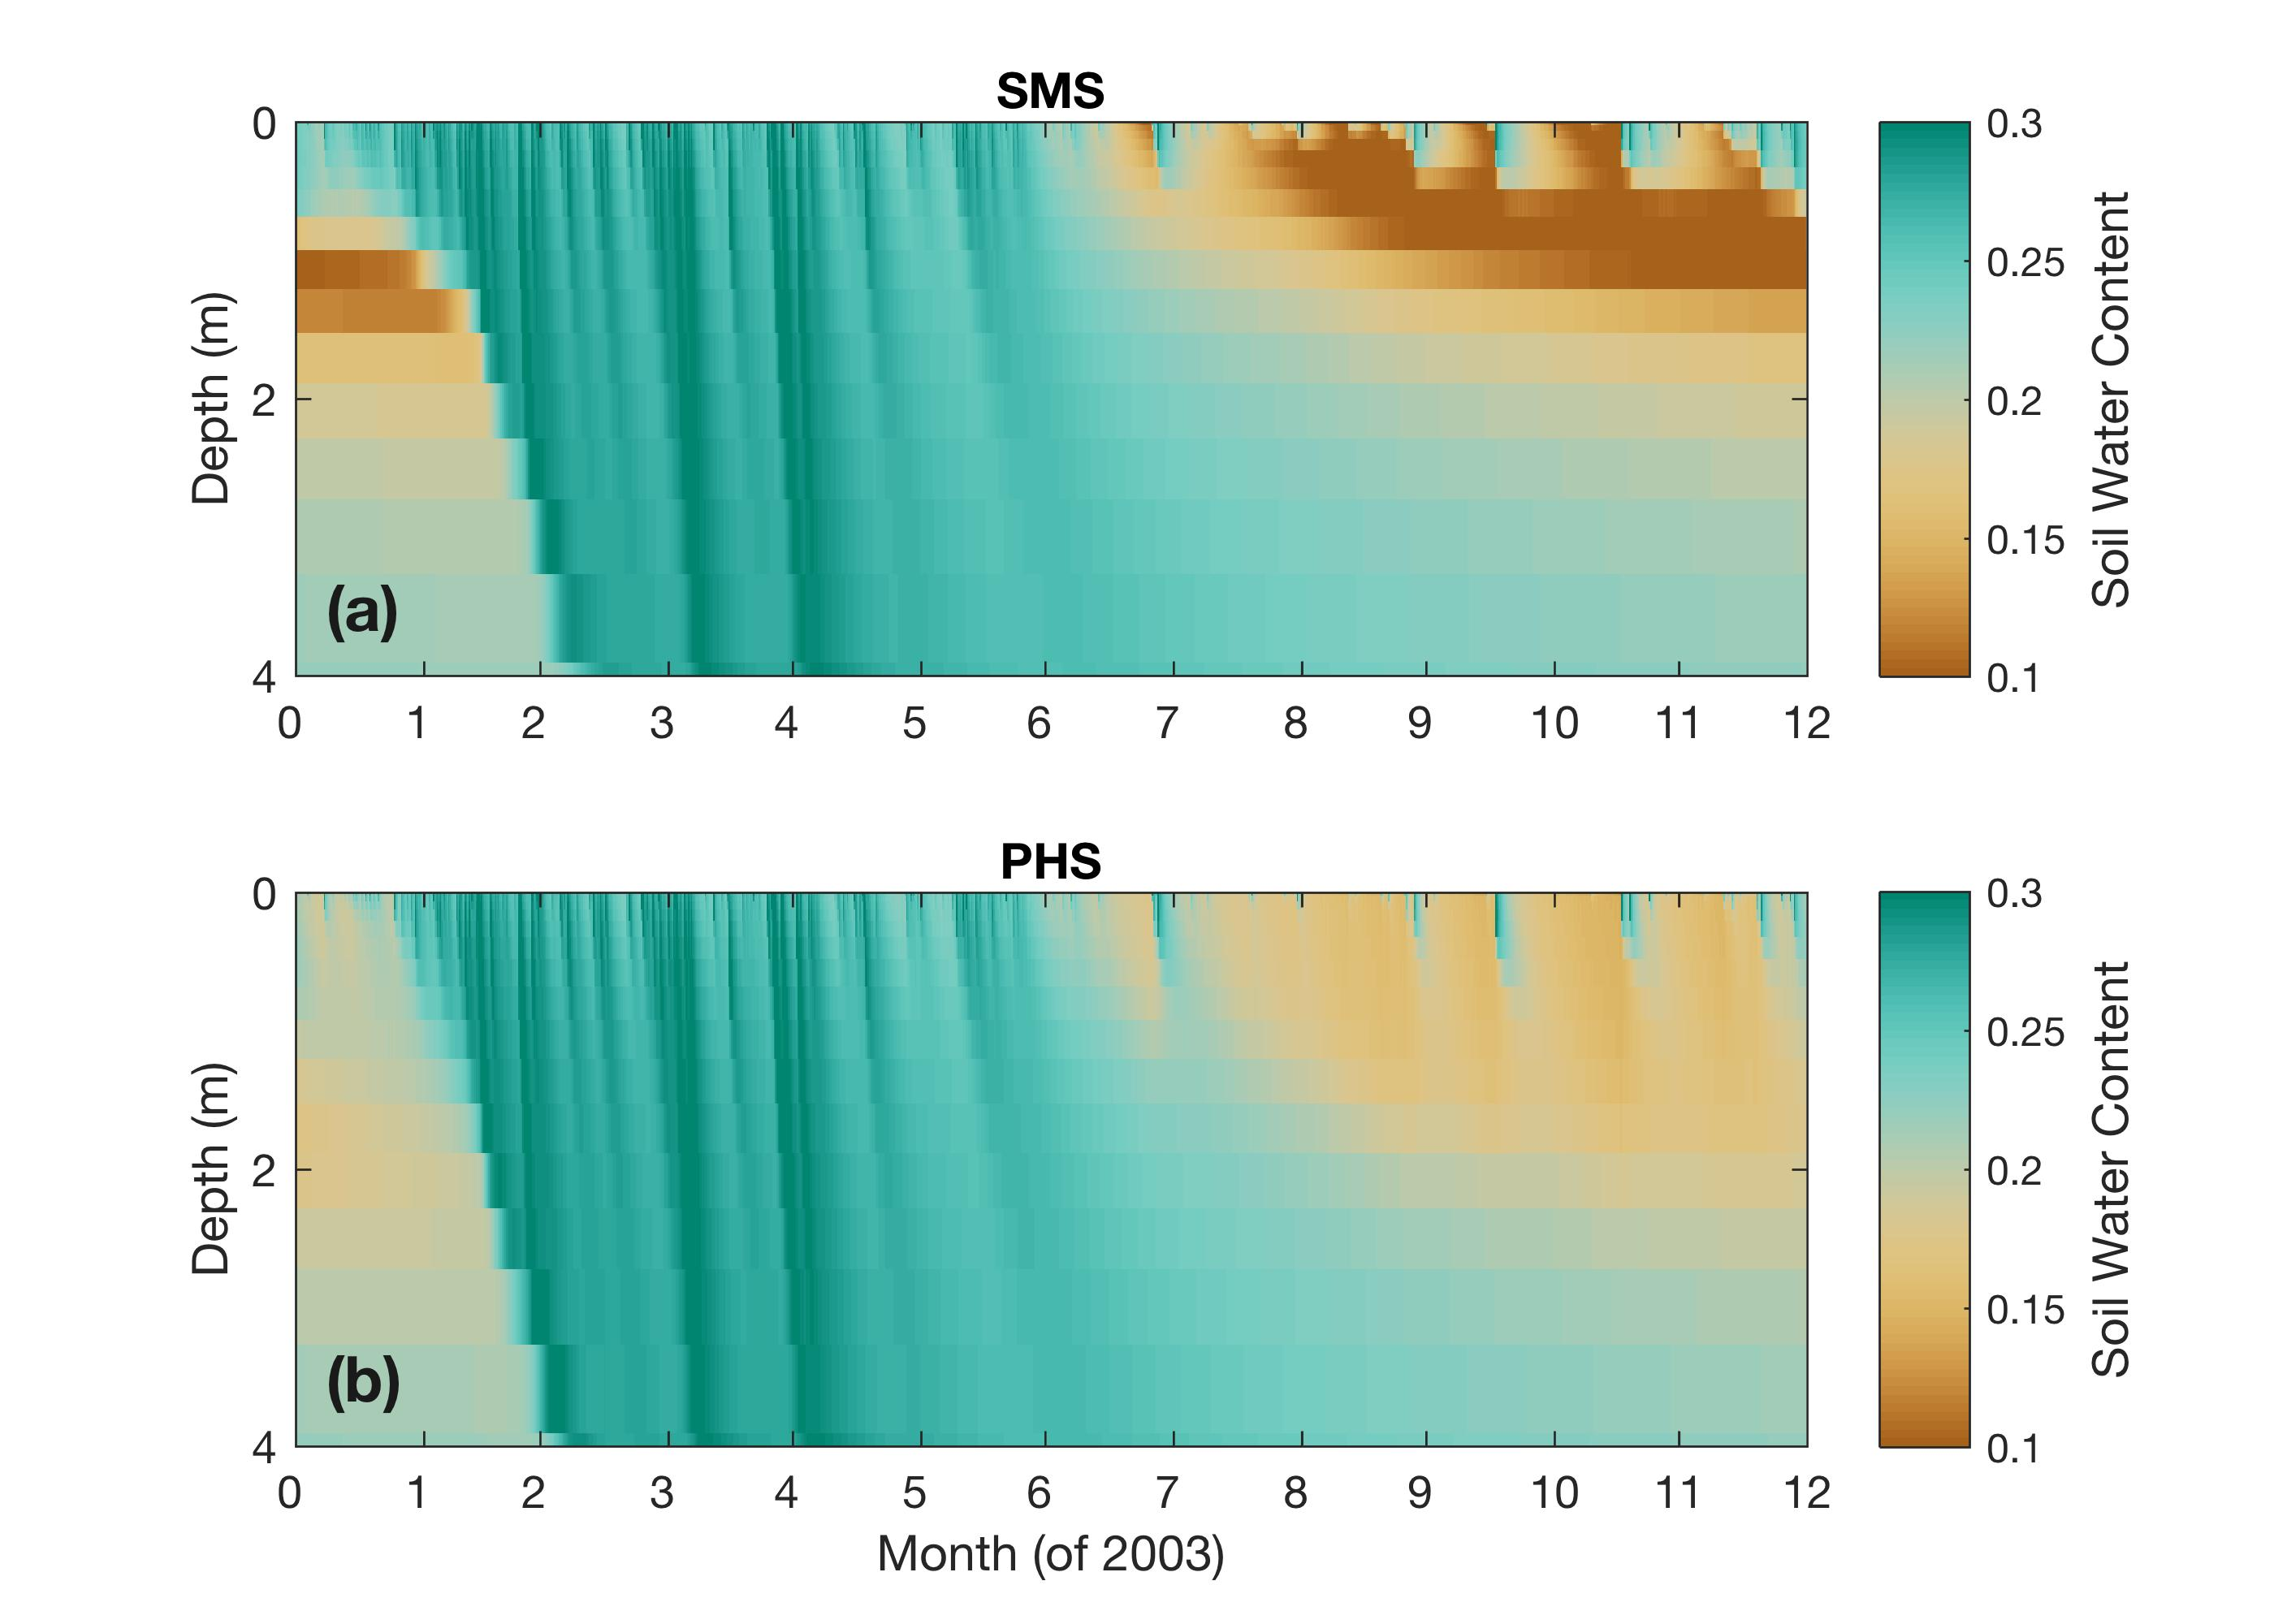
\includegraphics[width=30pc]{suppsmp.jpg}
     \caption{Vertical profile of soil water content (by volume) through time under ambient through-fall conditions, for
     (a) PHS, and 
     (b) SMS. }
     \label{supp:sm}
  \end{figure}
  
  \begin{figure}[h]
     \centering
     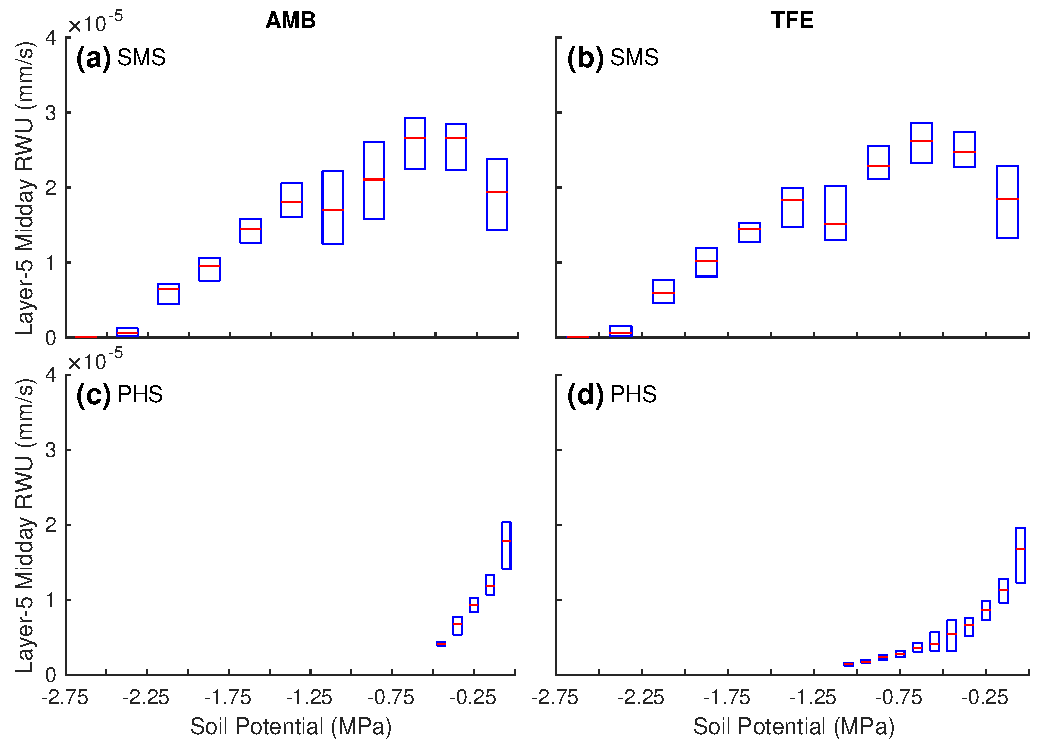
\includegraphics[width=30pc]{rwu.pdf}
     \caption{Binned boxplot of root water uptake versus soil potential for Soil Layer 5 (2002-3).
     Red lines mark the median, with boxes spanning the interquartile range.
     Bin widths are 0.25 MPa for SMS and 0.1 MPa for PHS.
     Soil Layer 5 is shown, because it is close enough to the surface (20 to 32 cm) to experience a significant range in soil potential, and it has a large root fraction (14.4\%, only Soil Layer 6 has a larger root fraction).
     Only midday (12h-14h) timesteps are used to highlight the relationship with soil potential.}
     \label{fig:rwu}
  \end{figure}
  \clearpage
  
    \begin{figure}[h]
     \centering
     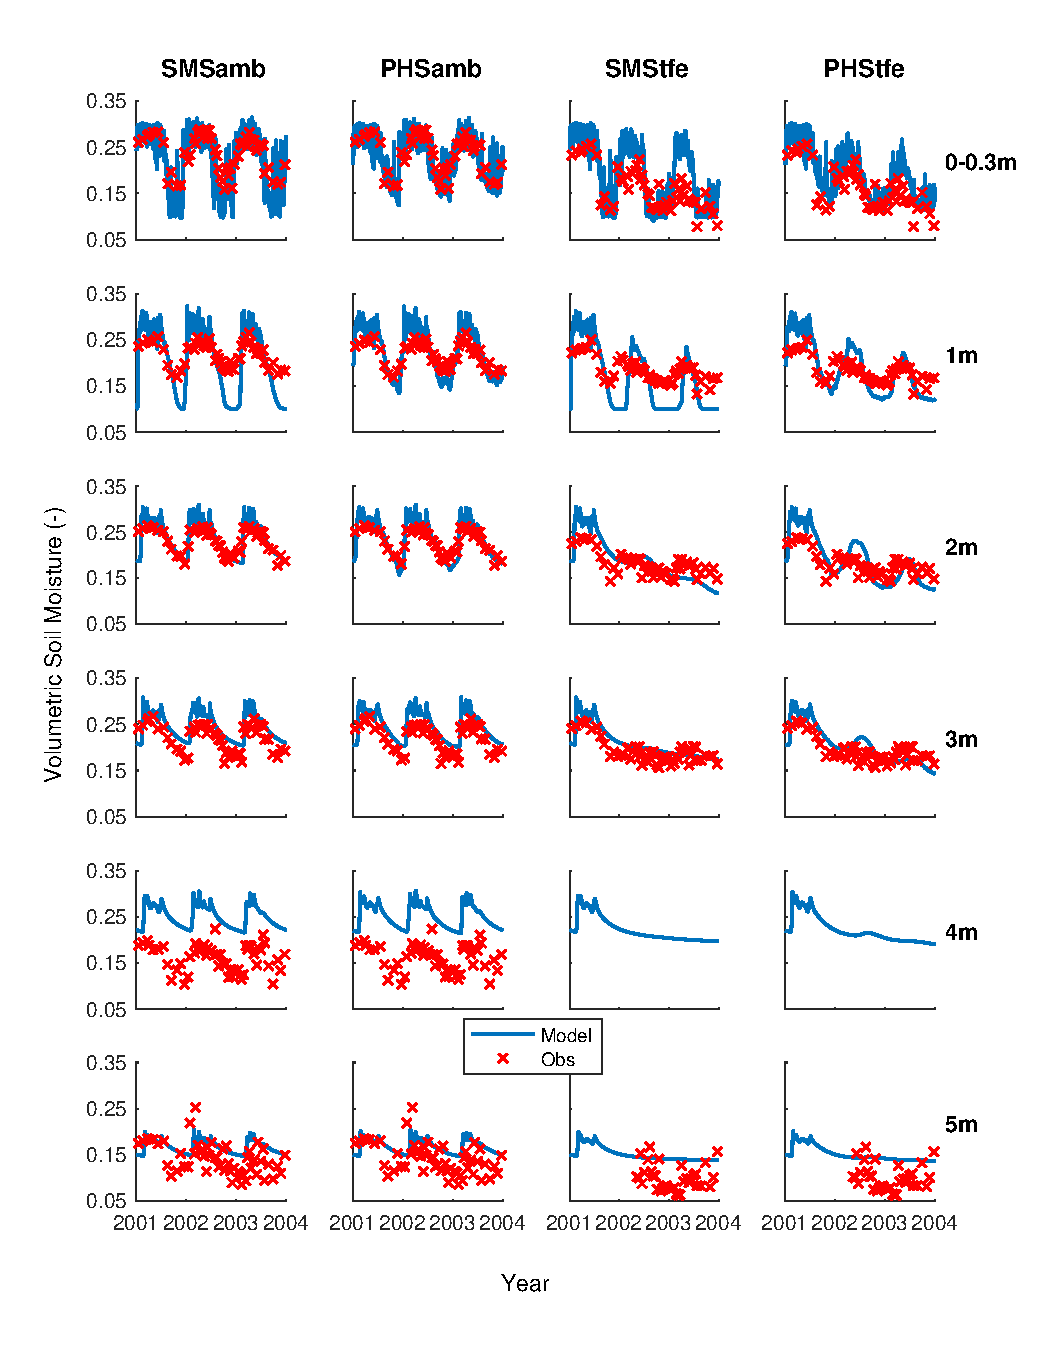
\includegraphics[width=30pc]{suppsm2.pdf}
     \caption{Time series of soil moisture by soil layer.
     Complements Figure 9.}
     \label{supp:sm2}
  \end{figure}
          \clearpage
          
     \begin{figure}[h]
     \centering
     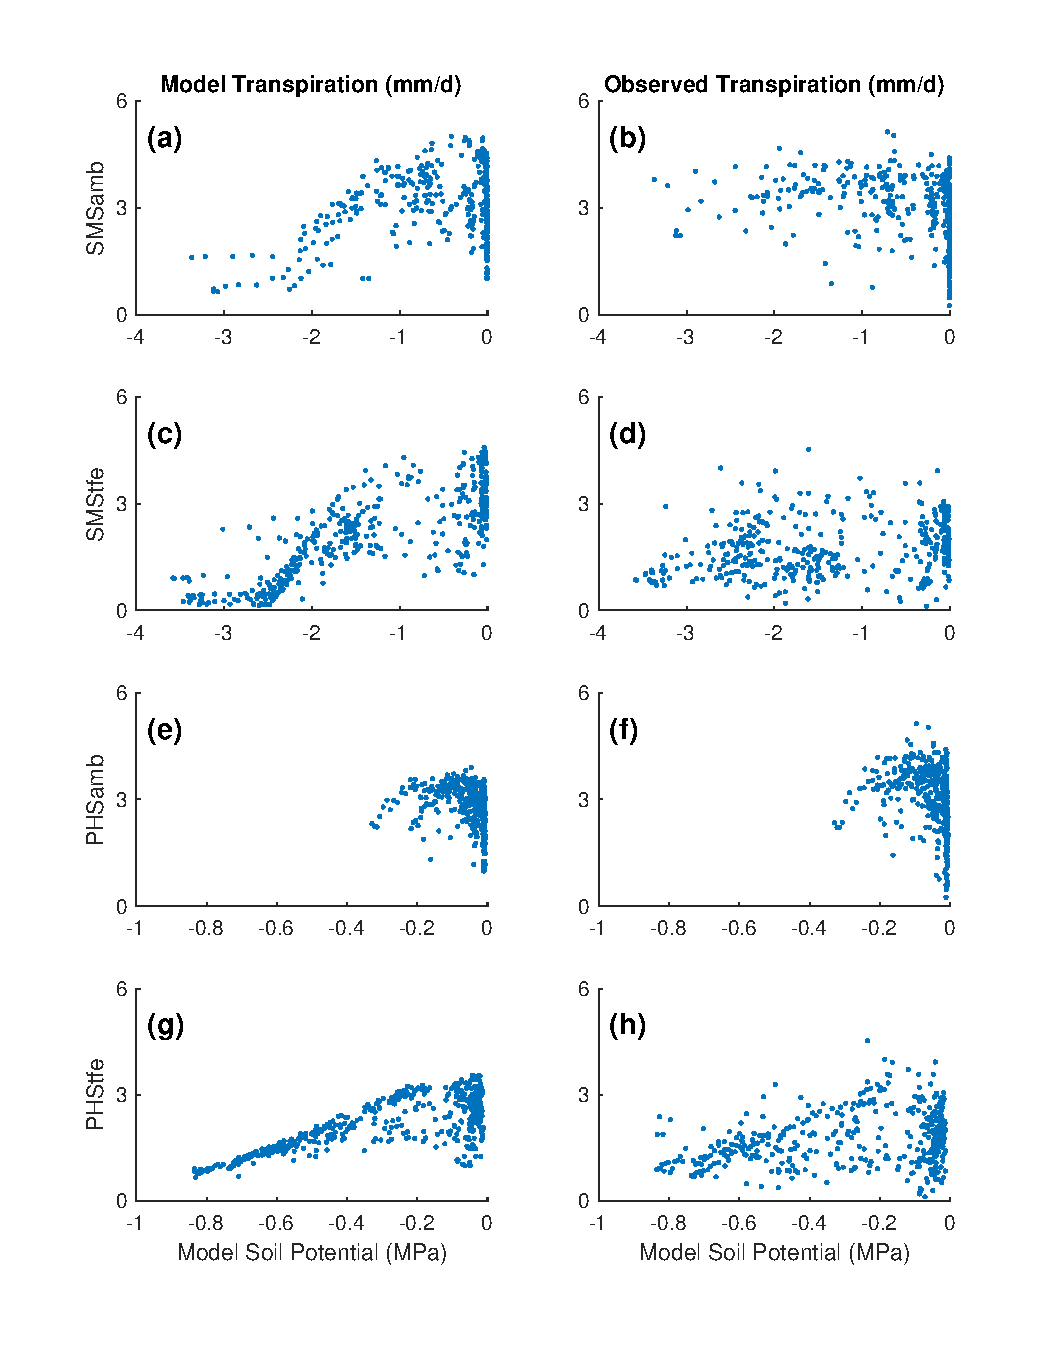
\includegraphics[width=30pc]{suppcool.pdf}
     \caption{Modeled (left column) and observed (right column) transpiration  vs. model soil potential.
     Complements Figure 13.}
     \label{supp:cool}
  \end{figure}
          \clearpage
          



%Delete all unused file types below. 
%Copy/paste for multiples of each file type as needed.

\end{document}